\section{Worksheet 6}
\subsection{Anti-Aliasing}
The pixel subdivision level is increased with the key \textbf{+} and decreased with the key \textbf{-}.\\
The array jitters contains an array of two dimentionals vector, which are random displacements of the coordinates of the lower left corner of the pixel.\\
If we have a subdivision level $s$ then function compute\_jitters will generate $s^2$ jitters. 
To reomove the aliasing artifacts we modify the compute pixel function that we made some worksheets before so that it casts a ray through all the jittered position of the pixels and then we return the averaged color computed from all the jittered positions.
\begin{lstlisting}
float3 RayCaster::compute_pixel(unsigned int x, unsigned int y) const
{
	Camera* camera = scene->get_camera();
	float2 coords = make_float2(lower_left.x + win_to_ip.x * x, lower_left.y + win_to_ip.y * y);
	float3 color = make_float3(0.0f);
	
	for (int i = 0; i < jitter.size(); i++) {
		Ray ray = camera->get_ray(coords+jitter[i]);
		
		HitInfo hit = HitInfo();
		bool has_hit = scene->closest_hit(ray, hit);
		if (has_hit) {
			color=color+ get_shader(hit)->shade(ray, hit);
		}
		else {
			color = color + get_background(ray.direction);
		}
	}
	return color / jitter.size();
}
\end{lstlisting}
As we can see from table \ref{table:time_comparison}  the rendering time seems to increase linearly with the subdivision level.
\begin{table}[H]
	\centering
	\begin{tabular}{|l|l|}
		\hline
		\textbf{Subdivision Level} & \textbf{Rendering Time} \\ \hline
		\textbf{1}                 & 2.401s                  \\ \hline
		\textbf{4}                 & 8.994s                  \\ \hline
		\textbf{9}                 & 21.63s                  \\ \hline
		\textbf{16}                & 36.325s                 \\ \hline
	\end{tabular}
	\caption{Comparison between subdivision level and rendering times}
	\label{table:time_comparison}
\end{table}
From figure \ref{fig:subdivison_comparison} we can see the differences between a subdivision level of 1, 4 and 9 are pretty noticeable. However increasing even more the subdivision level doesn't seem to provide any noticeable difference.
\begin{figure}[H]
	\centering
	\subfloat[\centering Subdivision level 1]{{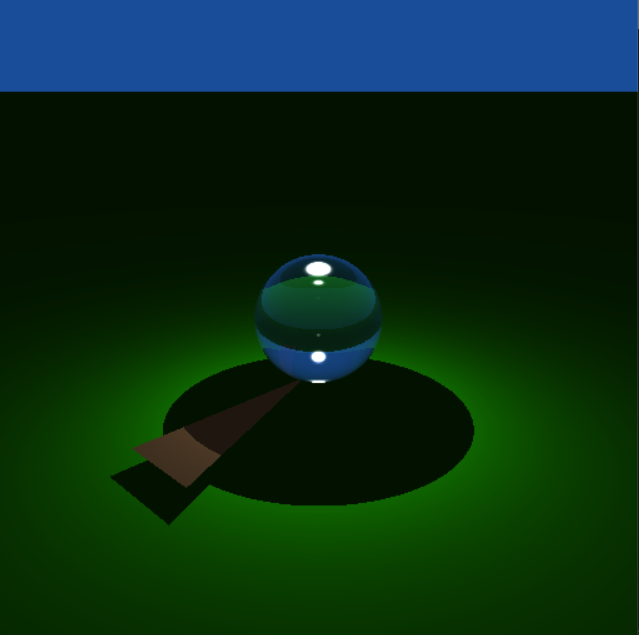
\includegraphics[width=5cm]{images/worksheet_6/subdivision_1} }}%
	\qquad
	\subfloat[\centering Subdivision level 4]{{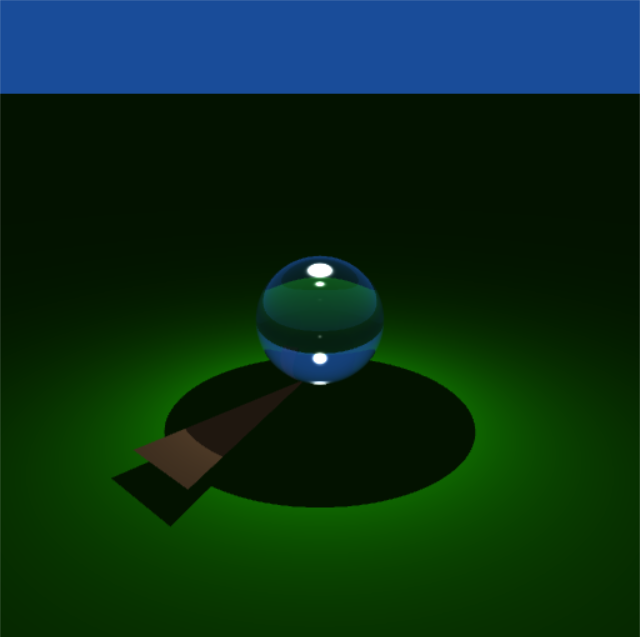
\includegraphics[width=5cm]{images/worksheet_6/subdivision_4} }}%
	\qquad
	\subfloat[\centering Subdivision level 9]{{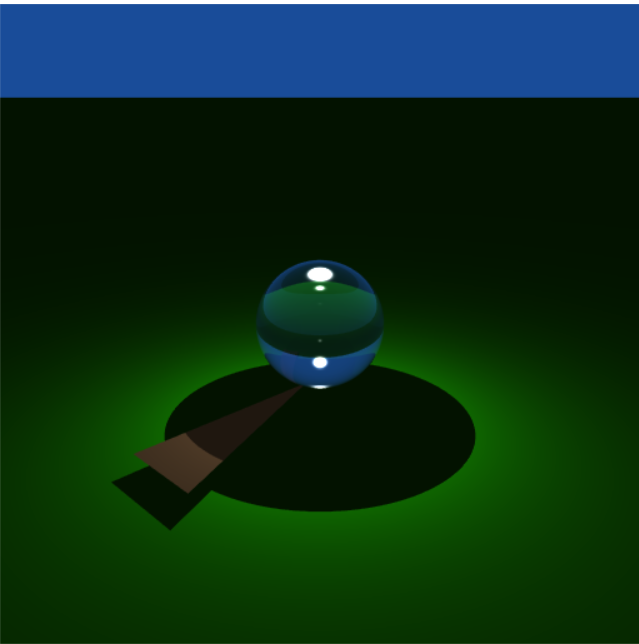
\includegraphics[width=5cm]{images/worksheet_6/subdivision_9} }}%
	\qquad
	\subfloat[\centering Subdivision level 16]{{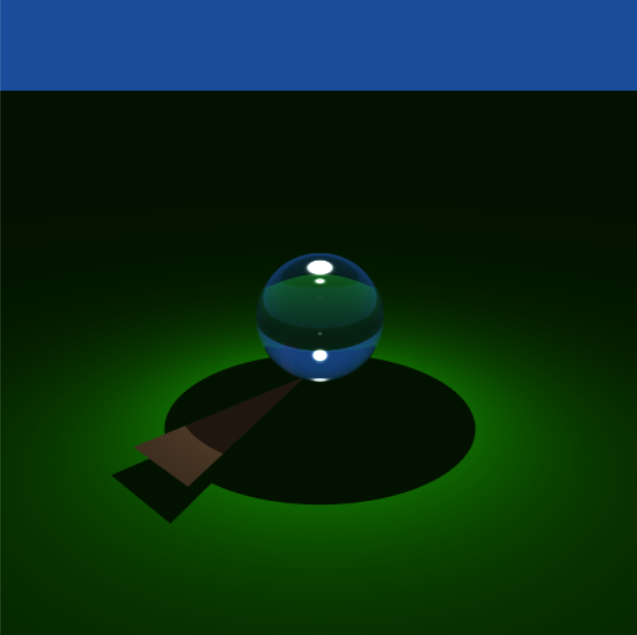
\includegraphics[width=5cm]{images/worksheet_6/subdivision_16} }}%	
	
	\caption{Comparison between different subdivision levels}%
	\label{fig:subdivison_comparison}%
\end{figure}

\subsection{Progressive path tracing}
To enable indirect illumination we have to implement the functions optix::float3 sample\_cosine\_weighted and MCGlossy::shade.
\begin{lstlisting}
inline optix::float3 sample_cosine_weighted(const optix::float3& normal)
{
	//return optix::make_float3(0.0f);
	// Get random numbers
	double epsilon_1 = mt_random_half_open();
	double epsilon_2 = mt_random_half_open();
	// Calculate new direction as if the z-axis were the normal
	float teta = acos(sqrt(1 - epsilon_1));
	float phi = 2 * M_PIf * epsilon_2;
	optix::float3 w = optix::make_float3(cos(phi)*sin(teta),sin(phi)*sin(teta),cos(teta));
	// Rotate from z-axis to actual normal and return
	rotate_to_normal(normal,w);
	return w;
}

float3 MCGlossy::shade(const Ray& r, HitInfo& hit, bool emit) const
{
	if(hit.trace_depth >= max_depth)
	return make_float3(0.0f);
	float3 rho_d = get_diffuse(hit);
	float3 result = make_float3(0.0f);
	
	float probability = (rho_d.x + rho_d.y + rho_d.z) / 3;
	float epsilon = mt_random_half_open();
	float3 L_indirect = make_float3(0.0f);
	if (epsilon < probability) {
		float3 w_j = sample_cosine_weighted(hit.shading_normal);
		HitInfo indirect_hit;
		indirect_hit.trace_depth = hit.trace_depth + 1;
		Ray new_ray = Ray(hit.position, w_j, 0, pow(10,-4),RT_DEFAULT_MAX);
		tracer->trace_to_closest(new_ray,indirect_hit);
		L_indirect = rho_d * shade_new_ray(new_ray, indirect_hit, false);
		L_indirect = L_indirect / probability;
	}
	return result + Lambertian::shade(r,hit,emit)+L_indirect;
}
\end{lstlisting}
In figure \ref{fig:ambient_light} you can see a rendering of the conrnell box with ambient lighting and indirect illuminations obtained with 300 samples per pixels.	
\begin{figure}[H]
	\centering
	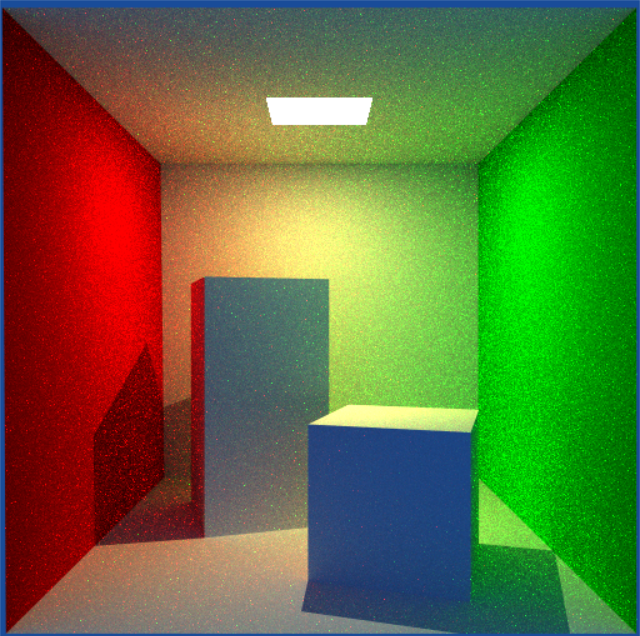
\includegraphics[scale=\imagescale]{images/worksheet_6/ambient_light}
	\caption{Cornell Box with indirect illumination}
	\label{fig:ambient_light}
\end{figure}